\documentclass[areasetadvanced]{scrartcl}

\usepackage[utf8]{inputenc}
\usepackage[T2A]{fontenc}
\usepackage[english,russian]{babel}
\usepackage{xcolor}

\usepackage[footskip=1cm,left=25mm, right=15mm, top=20mm, bottom=20mm]{geometry}
\usepackage{setspace}
\usepackage{amsmath, amssymb} 
\usepackage{graphicx}
\usepackage{tikz}
\usetikzlibrary{arrows.meta}
\usepackage{float}
\usepackage{dashrule}
\usepackage{fancyhdr} 
\usepackage{hyperref} 
\usepackage{parskip}
\usepackage{textcomp, enumitem}
\usepackage{indentfirst}
\usepackage{graphicx}
\usepackage{algorithm}
\usepackage{algpseudocode}
\usepackage{array} 
\usepackage{geometry}
\usepackage{afterpage}
\usepackage{minted}
\setcounter{secnumdepth}{3} 
\setcounter{tocdepth}{3}    
\usepackage{listings} 
\usepackage{booktabs}
\usepackage{paracol} % параллельные колонки (левая/правая)

\newcommand{\icon}[1]{\includegraphics[height=1.2em]{#1}}

\tikzstyle{block} = [rectangle, rounded corners, minimum width=3cm, minimum height=1cm, text centered, draw=black, fill=lightgray]

\setkomafont{sectioning}{\normalfont\bfseries} 
\setkomafont{section}{\normalfont\Large\bfseries}
\setkomafont{subsection}{\normalfont\large\bfseries}
\setkomafont{subsubsection}{\normalfont\large\bfseries}
\setkomafont{paragraph}{\normalfont\large\bfseries} 
\newcommand{\twosideheading}[2]{%
  \noindent
  \begin{minipage}[t]{0.5\textwidth}\raggedright\small #1\end{minipage}%
  \begin{minipage}[t]{0.5\textwidth}\raggedleft\Large\bfseries #2\end{minipage}\\[-0.2em]
  \hrule
  \vspace{0.8em}
}
\lstset{
  language=Haskell,
  basicstyle=\ttfamily\small,
  keywordstyle=\color{blue}\bfseries,
  stringstyle=\color{red},
  commentstyle=\color{green!70!black},
  numbers=left,
  numberstyle=\tiny,
  stepnumber=1,
  numbersep=10pt,
  showstringspaces=false,
  breaklines=true,
  frame=single
}

\lstdefinelanguage{Lua}{
    keywords={function, end, if, then, else, elseif, for, while, do, repeat, until, break, return, local, and, or, not, true, false, nil},
    keywordstyle=\color{blue}\bfseries,
    stringstyle=\color{red},
    commentstyle=\color{green!70!black},
    morestring=[s]{"}{"},
    morestring=[s]{'}{'},
    morecomment=[l]{--},
    morecomment=[s]{--[[}{]]},
    basicstyle=\ttfamily\small,
    numbers=left,
    numberstyle=\tiny,
    stepnumber=1,
    numbersep=10pt,
    showstringspaces=false,
    breaklines=true,
    frame=single
}

\lstdefinestyle{py}{
    language=Python,
    basicstyle=\ttfamily\small,
    keywordstyle=\color{blue}\bfseries,
    stringstyle=\color{red},
    commentstyle=\color{green!70!black},
    numbers=left,
    numberstyle=\tiny,
    stepnumber=1,
    numbersep=10pt,
    showstringspaces=false,
    breaklines=true,
    frame=single
}

\setlength{\parindent}{1.25cm}
\setcounter{tocdepth}{3}
\begin{document}
\sloppy
	\thispagestyle{empty}
	\begin{center}
		\large{МИНОБРНАУКИ РОССИИ} \par
		\vspace{0.3cm}
		\normalsize
		{ФЕДЕРАЛЬНОЕ ГОСУДАРСТВЕННОЕ АВТОНОМНОЕ ОБРАЗОВАТЕЛЬНОЕ УЧРЕЖДЕНИЕ ВЫСШЕГО ОБРАЗОВАНИЯ} \par
		\vspace{0.3cm}
		\textbf{\guillemotleft САНКТ-ПЕТЕРБУРГСКИЙ ПОЛИТЕХНИЧЕСКИЙ}
		\textbf{УНИВЕРСИТЕТ ПЕТРА ВЕЛИКОГО\guillemotright} \par
		\vspace{0.3cm}
		{Институт компьютерных наук и кибербезопасности}\par
		{Высшая школа технологий искусственного интеллекта}\par
	\end{center}
	\vfill
	\begin{center}
		{\large Отчёт по дисциплине \guillemotleft Генетические алгоритмы\guillemotright}\par
		\vspace{1cm}
		\Huge Практическая работа №4\par
		\vspace{0.5cm}
		{\huge \guillemotleft Генетическое программирование\guillemotright \\
        Вариант №17}\par
	\end{center}
	\vfill
	\begin{flushleft}
		Студент: \hspace{1.8cm} \rule[0pt]{2.5cm}{0.5pt}\hfill Салимли Айзек Мухтар Оглы\par
		\vspace{1.5cm}
		Преподаватель: \hspace{0.55cm} \rule[0pt]{2.5cm}{0.5pt}\hfill  Большаков Александр Афанасьевич
	\end{flushleft}
	\vspace{0.5cm}
	\begin{flushright}
		\guillemotleft \rule[0pt]{0.8cm}{0.5pt}\guillemotright \rule[0pt]{2cm}{0.5pt} 20\rule[0pt]{0.5cm}{0.5pt} г.
	\end{flushright}
	\vfill
	\begin{center}
		Санкт-Петербург, 2025
	\end{center}
	\newpage
	\tableofcontents
	\newpage

\section*{Введение}
\addcontentsline{toc}{section}{Введение}
Генетические алгоритмы относятся к классу эволюционных методов оптимизации и активно применяются для решения сложных задач, где традиционные подходы оказываются малоэффективными. Эти алгоритмы вдохновлены природными
процессами естественного отбора и наследственности, что позволяет им эффективно
исследовать пространство решений и находить близкие к оптимальным результаты.
В данной лабораторной работе реализован эволюционный алгоритм на основе генетического программирования для аппроксимации функции.

\newpage
\section{Постановка задачи}

В лабораторной работе требовалось:
\begin{enumerate}
  \item Разработать эволюционный алгоритм, реализующий генетическое программирование (ГП) для нахождения (символьной регрессии) заданной по варианту функции.
  \begin{itemize}
    \item Структура для представления программы — древовидное представление.
    \item Терминальное множество: переменные \(x_1,\dots,x_n\) и эфемерные случайные константы.
    \item Функциональное множество: \(+\), \(-\), \(\ast\), \(/\), \(\sin()\), \(\cos()\), \(\exp()\), возведение в степень \((\hat{\ }\;\text{или}\;^{})\).
    \item Фитнесс-функция — мера близости между реальными значениями выхода и требуемыми, основанная на сумме квадратов ошибок (SSE).
  \end{itemize}
  \item Представить графически найденное решение на каждой 10-й итерации и в конце работы алгоритма.
  \item Сравнить найденное решение с представленным в условии задачи.
\end{enumerate}

\textbf{Исходные данные}

\begin{itemize}
  \item Функция:
  \[
    f_{1a}(x) \;=\; \sum_{i=1}^{n} i \cdot x_i^2
  \]
  \item Количество переменных: \(N = 9\).
  \item Промежуток исследования: \(x_i \in [\, -5.12,\; 5.12 \,]\).
\end{itemize}

\newpage
\section{Теоретические сведения}
\subsection{Терминальное множество}

Терминальное множество включает в себя "листья" дерева программы — элементы, которые не принимают аргументов. К ним относятся:
\begin{enumerate}
  \item Внешние входы в программу: переменные (в данной работе \(x_1, x_2, x_3, x_4\)).
  \item Используемые в программе константы: числовые значения, которые могут быть как предопределёнными, так и случайно генерируемыми (эфемерные случайные константы).
  \item Функции, которые не имеют аргументов.
\end{enumerate}

\subsection{Функциональное множество}

Функциональное множество состоит из операторов и функций, которые являются внутренними узлами дерева и обрабатывают значения от дочерних узлов. В данной работе оно включает:
\begin{itemize}
  \item \textbf{Арифметические функции:} сложение \((+)\), вычитание \((-)\), умножение \((\cdot)\), деление \((/)\).
  \item \textbf{Трансцендентные функции:} синус \(\sin\), косинус \(\cos\), экспонента \(\exp\).
  \item \textbf{Другие функции:} возведение в степень \((\hat{\ }\; \text{или } ^{})\).
\end{itemize}

\subsection{Древовидные структуры}

Древовидная форма представления является классической для ГП. Программа представляется в виде дерева, где внутренние узлы — это функции из функционального множества, а листья (терминальные узлы) — это переменные и константы из терминального множества. Такая структура позволяет гибко работать с выражениями различной длины и сложности.

\subsection{Инициализация древовидных структур}

Начальная популяция деревьев создаётся с помощью двух основных методов:
\begin{itemize}
  \item \textbf{Полный (full):} генерируются деревья, у которых все листья находятся на максимально заданной глубине.
  \item \textbf{Растущий (grow):} генерируются деревья неправильной формы, где терминалы могут находиться на разной глубине, не превышающей максимальную.
\end{itemize}
На практике часто используется их комбинация (\emph{ramped half-and-half}) для обеспечения разнообразия структур в начальной популяции.

\subsection{Кроссинговер на древовидных и графоподобных структурах}

В генетическом программировании для графоподобных структур применяются два основных вида оператора кроссинговера. Эти методы комбинируют генетический материал из двух родительских программ путём обмена их частями.

\subsection{Кроссинговер подграфов}

Этот способ аналогичен кроссинговеру поддеревьев, который используется для древовидных структур. Процесс обмена происходит следующим образом:
\begin{enumerate}
  \item В каждой родительской программе (графе) случайным образом выбирается множество смежных узлов, образующих подграф.
  \item Производится обмен этими двумя подграфами между родительскими особями, в результате чего создаются две новые дочерние программы.
\end{enumerate}
Этот метод позволяет обмениваться целыми функциональными блоками программы.

\subsection{Линейный кроссинговер}

Второй тип кроссинговера оперирует на уровне линейных сегментов кода внутри узлов графа:
\begin{enumerate}
  \item В каждом из родительских графов выбирается один узел.
  \item Внутри линейной программы этого узла выбирается сегмент кода, который определяется случайной начальной позицией и случайной длиной.
  \item Происходит обмен этими линейными сегментами между родителями.
  \item Если размер хотя бы одного из потомков превышает установленный порог, результаты кроссинговера могут быть аннулированы, и вместо этого выполняется обмен сегментами меньшей длины.
\end{enumerate}
Обычно данный вид кроссинговера выполняется с определённой вероятностью, например, \(P_l = 0.1\).

Как правило, в процессе эволюции для графоподобных структур используются оба типа кроссинговера для обеспечения как обмена крупными блоками (кроссинговер подграфов), так и более тонкой настройки внутри этих блоков (линейный кроссинговер).

\subsection{Кроссинговер поддеревьев (Subtree Crossover) для древовидных структур}

Кроссинговер поддеревьев является основным генетическим оператором, используемым для рекомбинации в генетическом программировании (ГП), когда программы представлены в виде древовидных структур. Он создаёт новые дочерние программы (потомков) путём обмена случайно выбранными поддеревьями между двумя родительскими программами.

\subsubsection{Алгоритм выполнения}
Процесс кроссинговера поддеревьев выполняется в несколько шагов:
\begin{enumerate}
  \item \textbf{Выбор двух родителей.} Из текущей популяции для скрещивания выбираются две особи (программы-деревья).
  \item \textbf{Выбор точки скрещивания в каждом родителе.} В каждом из двух родительских деревьев случайным образом выбирается один узел. Этот узел становится корнем поддерева, которое будет участвовать в обмене. Точкой скрещивания может быть как функциональный узел (внутренний узел дерева), так и терминальный узел (лист).
  \item \textbf{Обмен поддеревьями.} Поддерево, начинающееся в точке скрещивания первого родителя, меняется местами с поддеревом из точки скрещивания второго родителя.
  \item \textbf{Создание потомков.} В результате этого обмена создаются две новые дочерние программы. Каждая из них содержит часть генетического материала от одного родителя и <<привитое>> поддерево от другого.
\end{enumerate}

\subsubsection{Пример}
Рассмотрим две родительские программы, представленные в виде математических выражений:
\[
\text{Родитель 1: } \min\bigl(x - 6,\; x + y\cdot 2\bigr), \qquad
\text{Родитель 2: } 3\cdot x + \frac{y}{2}.
\]
Процесс кроссинговера:
\begin{itemize}
  \item В Родителе 1 в качестве точки скрещивания выбирается узел \((+)\). Поддерево, соответствующее этому узлу, — это выражение \(x + y\cdot 2\).
  \item В Родителе 2 в качестве точки скрещивания выбирается узел \((\cdot)\). Соответствующее поддерево — \(3\cdot x\).
\end{itemize}
После обмена этими поддеревьями получаются два потомка:
\[
\text{Потомок 1: } \min\bigl(x - 6,\; 3\cdot x\bigr), \qquad
\text{Потомок 2: } \bigl(x + y\cdot 2\bigr) + \frac{y}{2}.
\]

\subsection{Выполнение мутации на древовидных структурах}

Оператор мутации вносит случайные изменения в особь. Основные виды для деревьев:
\begin{itemize}
  \item \textbf{Узловая:} замена одного узла на другой того же типа.
  \item \textbf{Усекающая:} замена целого поддерева на один случайный терминал.
  \item \textbf{Растущая:} замена случайного узла на новое, случайно сгенерированное поддерево.
\end{itemize}

\subsection{Фитнесс-функция в генетическом программировании}

В ГП фитнесс-функция почти всегда определяет меру ошибки программы. Она вычисляется на наборе тестовых данных и показывает, насколько сильно выходные значения программы отличаются от эталонных. Часто используется сумма квадратов ошибок (SSE). Цель эволюции — минимизировать эту ошибку, что эквивалентно максимизации фитнесс-функции, например:
\[
F \;=\; \frac{1}{1 + \mathrm{SSE}}.
\]

\newpage
\section{Программная реализация}
Программа решает задачу символьной регрессии для
\[
f_{1a}(\mathbf{x})=\sum_{i=1}^{n} i\,x_i^2,\quad x_i\in[-5.12,\,5.12],
\]
используя эволюционный алгоритм с древовидным представлением, терминалами \(\{x_1,\dots,x_9,\text{ERC}\}\) и функциональным множеством \(\{+, -, *, /, \sin, \cos, \exp, \hat{}\}\).
Алгоритм минимизирует \(\mathrm{SSE}\) (с дополнительной парсимонией по размеру дерева), выводит дерево лучшей особи через Graphviz, а также графики сходимости, средней длины программ и распределения ошибок.

\subsection{Импорт и конфигурация}
Основные импорты: \texttt{math}, \texttt{random}, \texttt{numpy}, \texttt{matplotlib.pyplot}, \texttt{dataclasses}, \texttt{typing}; опционально \texttt{graphviz} (\texttt{GRAPHVIZ\_AVAILABLE}).\\
\textbf{Константы (CONFIG):} \(\texttt{N\_VARS}=9\), \(\texttt{DOMAIN}=(-5.12,5.12)\), \(\texttt{POP\_SIZE}\), \(\texttt{GENERATIONS}\), турнир \(k=\texttt{TOURNAMENT\_K}\), вероятности операторов (\(\texttt{P\_CROSS},\texttt{P\_MUT\_NODE},\texttt{P\_MUT\_SHRINK},\texttt{P\_MUT\_GROW}\)), предельные глубины (\(\texttt{MAX\_INIT\_DEPTH},\texttt{MAX\_TREE\_DEPTH}\)), диапазон ERC и штраф за сложность \(\lambda=\texttt{LAMBDA\_COMPLEXITY}\).

\subsection{Защищённые операции (числовая стабильность)}
\verb|p_div| (защищённое деление), \verb|p_pow| (защищённая степень: клип показателя, модуль для нецелых), \verb|p_exp| (клип аргумента), \verb|p_sin|, \verb|p_cos|.\\
Назначение: предотвратить \(\mathrm{NaN}/\infty\) и переполнения при вычислении деревьев.

\subsection{Примитивы и узлы дерева}
\verb|@dataclass Primitive|: имя, арность, функция. Словарь \verb|FUNCTIONS| для \((+, -, *, /, \sin, \cos, \exp, \hat{} )\).\\
\verb|@dataclass Terminal|: терминал-переменная (\verb|kind='var'|, \verb|index|) или ERC (\verb|kind='erc'|, \verb|value|), метод \verb|eval|.\\
\verb|@dataclass Node|: \verb|prim| \(\in\) \{\verb|Primitive|, \verb|Terminal|\}, \verb|children|; служебные методы: \verb|is_function|/\verb|is_terminal|, \verb|copy|, \verb|depth|, \verb|size|, \verb|eval| (векторизованная оценка на \(X\)), \verb|to_string| (инфиксная запись).

\subsection{Инициализация деревьев}
\verb|random_terminal| (переменная или ERC), \verb|random_function| (по арности), \verb|generate_full|, \verb|generate_grow|, \verb|generate_ramped|.\\
Метод \emph{ramped half-and-half}: баланс разнообразия форм и глубин в начальной популяции.

\subsection{Генетические операторы}
\textbf{Селекция.} \verb|tournament(pop, fitness, k)| — турнирная селекция; минимизируется \(\mathrm{SSE}\).\\
\textbf{Кроссинговер.} \verb|all_nodes_with_parents| собирает узлы с родителями; \verb|subtree_crossover| обменивает случайные поддеревья (с проверкой \verb|MAX_TREE_DEPTH|).\\
\textbf{Мутации.} \verb|mutate_node_replace| (замена функции/терминала на однотипный), \verb|mutate_shrink| (усечение: функция \(\to\) терминал), \verb|mutate_grow| (вставка случайного поддерева ограниченной глубины).

\subsection{Целевая функция и датасеты}
 \verb|target_function(X)|: векторизованно считает \(f_{1a}\) на матрице \(X\). \verb|make_dataset| генерирует обучающую и валидационную выборки в \([-5.12,5.12]^9\).

\subsection{Фитнесс-функция}
 \verb|fitness_sse(ind, X, y)|: \(\mathrm{SSE}=\sum(y-\hat{y})^2\) с парсимонией \(+\lambda\cdot\text{size}^2\); защита от \(\mathrm{NaN}/\infty\).

\subsection{Визуализация дерева (Graphviz)}
 \verb|plot_tree_graphviz(root, filename, title)|: строит \verb|graphviz.Digraph|; функциональные узлы — эллипсы, терминалы/константы — прямоугольники; сохраняет \texttt{PNG}. Используется каждые 10 поколений и в конце.

\subsection{Главный эволюционный цикл}
 \verb|evolve()|:
\begin{enumerate}
  \item Генерация обучающего/валидационного наборов.
  \item Инициализация популяции \verb|generate_ramped|.
  \item Для каждого поколения: оценка \(\mathrm{SSE}\), элитизм (\verb|ELITE|), селекция, кроссинговер, мутации; обновление лучшей особи. Ведётся журнал \verb|best_hist| (лучший \(\mathrm{SSE}\)) и \verb|avg_size_hist| (средний размер дерева).
  \item Каждые \verb|PLOT_EVERY| поколений — \verb|plot_tree_graphviz|.
  \item Финальный отчёт и три графика: (i) сходимость \(\mathrm{SSE}\), (ii) средняя длина программ, (iii) гистограмма остатков на валидации.
\end{enumerate}

\subsection{Выходные визуализации}
\begin{itemize}
  \item \textbf{Сходимость:} линия \(\min\mathrm{SSE}\) по поколениям — контроль прогресса оптимизации.
  \item \textbf{Средняя длина программ:} \(\frac{1}{|\mathcal{P}|}\sum\text{size}(\text{индивид})\) — мониторинг bloat.
  \item \textbf{Распределение ошибок:} гистограмма \(r=y-\hat{y}\) на валидации — проверка смещения/разброса.
  \item \textbf{Дерево решения:} \texttt{tree\_gen\_\#}.png (срезы) и \texttt{tree\_final.png} (финал).
\end{itemize}

\subsection{Ключевые параметры для тонкой настройки}
\begin{itemize}
  \item \textbf{Сложность/парсимония:} \verb|LAMBDA_COMPLEXITY|, \verb|MAX_TREE_DEPTH|.
  \item \textbf{Поиск:} \verb|POP_SIZE|, \verb|GENERATIONS|, \verb|TOURNAMENT_K|.
  \item \textbf{Баланс операторов:} \verb|P_CROSS|, \verb|P_MUT_NODE|, \verb|P_MUT_SHRINK|, \verb|P_MUT_GROW|.
  \item \textbf{Стохастика:} диапазон \verb|ERC_RANGE|.
\end{itemize}

\newpage
\section{Результаты}

Алгоритм был реализован на языке Python и запущен на \(120\) поколений для задачи символьной регрессии
\[
f_{1a}(\mathbf{x})=\sum_{i=1}^{9} i\,x_i^2,\qquad x_i\in[-5.12,\,5.12].
\]
Ниже приведены ключевые параметры запуска и сводные наблюдения по логам работы.

\paragraph{Параметры эксперимента}
\begin{itemize}
  \item Размер популяции: \(300\) особей.
  \item Количество поколений: \(120\).
  \item Вероятность кроссинговера: \(0.9\).
  \item Вероятности мутаций: узловая \(0.2\), усечение \(0.1\), рост \(0.2\).
  \item Метод отбора: турнирный, размер турнира \(k=5\).
  \item Элитизм: \(2\) лучшие особи переходят в следующее поколение.
  \item Ограничения структуры: начальная глубина до \(6\), максимальная глубина дерева \(16\).
  \item Парсимония: малый штраф за сложность \(\lambda=\texttt{LAMBDA\_COMPLEXITY}=10^{-4}\).
\end{itemize}

\paragraph{Анализ динамики фитнесса}
Оптимизация велась по сумме квадратов ошибок (SSE), при этом фитнесс интерпретировался как \(\displaystyle F = 1/(1+\mathrm{SSE})\).
По журналам видно характерную для ГП картину:
\begin{itemize}
  \item Уже на первых поколениях достигается заметное снижение \(\mathrm{SSE}\) за счёт быстрого распространения удачных фрагментов деревьев.
  \item В интервале примерно до \(50\)-го поколения наблюдается монотонное, но замедляющееся улучшение лучшего решения.
  \item Далее улучшения становятся редкими и небольшими; к \(\sim 90\)–\(100\) поколению \(\mathrm{SSE}\) стабилизируется на плато, что соответствует практически неизменному значению фитнесса.
  \item Средний фитнесс популяции растёт быстрее на ранних этапах и выходит на высокий стабильный уровень к завершающей трети эволюции, что указывает на успешное распространение «генетического материала» лучших особей механизмами отбора и кроссинговера.
\end{itemize}
Такая динамика подтверждает работоспособность поиска: алгоритм выходит из локальных минимумов и постепенно дорабатывает решение, пока не достигает зоны стагнации.

\paragraph{Анализ сложности программ (Bloat)}
Запуск демонстрирует типичное явление «вздутия» кода:
\begin{itemize}
  \item \textbf{Нейтральные замены лучшей особи.} Даже при почти неизменной \(\mathrm{SSE}\) структура лучшей программы заметно меняется от поколения к поколению: размер дерева то растёт, то падает, что свидетельствует о замене одной близкой по качеству программы на другую, зачастую более крупную. Это эффект ``\emph{survival of the fattest}'' — крупные деревья более устойчивы к деструктивным мутациям/кроссинговеру.
  \item \textbf{Рост среднего размера.} График средней длины программ показывает восходящий тренд в течение запуска: популяция аккумулирует ``интроны'' (участки, мало влияющие на выход), что увеличивает сложность без эквивалентного выигрыша в качестве после определённого момента времени.
\end{itemize}

\paragraph{Общий вывод по результатам}
Запуск можно считать успешным: алгоритм быстро нашёл решения с низкой ошибкой и стабилизировал качество к финалу эволюции. Одновременно отчётливо проявился \textbf{bloat}, что подчёркивает важность приёмов контроля сложности (усиление штрафа за размер, более жёсткие ограничения глубины, упрощение выражений) для получения не только точных, но и компактных формул.

\begin{figure}[H]
  \centering
  \includegraphics[width=0.51\linewidth]{img/tree_gen_10.png}
  \caption{Дерево 10-го поколения}
\end{figure}

\begin{figure}[H]
  \centering
  \includegraphics[width=0.51\linewidth]{img/tree_gen_20.png}
  \caption{Дерево 20-го поколения}
\end{figure}

\begin{figure}[H]
  \centering
  \includegraphics[width=0.51\linewidth]{img/tree_gen_50.png}
  \caption{Дерево 50-го поколения}
\end{figure}

\begin{figure}[H]
  \centering
  \includegraphics[width=0.51\linewidth]{img/tree_gen_70.png}
  \caption{Дерево 70-го поколения}
\end{figure}

\begin{figure}[H]
  \centering
  \includegraphics[width=0.51\linewidth]{img/tree_gen_100.png}
  \caption{Дерево 100-го поколения}
\end{figure}

\begin{figure}[H]
  \centering
  \includegraphics[width=0.51\linewidth]{img/tree_final.png}
  \caption{Финальное дерево}
\end{figure}

\begin{figure}[H]
  \centering
  \includegraphics[width=0.51\linewidth]{img/output.png}
  \caption{Сходимость алгоритма (лучший \(\mathrm{SSE}\) по поколениям)}
\end{figure}

\begin{figure}[H]
  \centering
  \includegraphics[width=0.51\linewidth]{img/output1.png}
  \caption{Средний размер дерева (число узлов) по поколениям}
\end{figure}

\begin{figure}[H]
  \centering
  \includegraphics[width=0.51\linewidth]{img/error.png}
  \caption{Распределение ошибок на валидации}
\end{figure}

\newpage
\section{Анализ исследования}
\paragraph{Качество аппроксимации и сходимость}
\begin{itemize}
  \item Алгоритм нашёл решения с низкой ошибкой на ранних поколениях, после чего демонстрировал постепенное улучшение.
  \item Снимки дерева лучшей особи на промежуточных этапах и финальная структура подтверждают, что улучшение шло за счёт замены и перестройки поддеревьев (структурная эволюция формулы).
\end{itemize}

\paragraph{Сложность программ (bloat)}
\begin{itemize}
  \item По графику среднего размера деревьев виден устойчивый рост сложности популяции: эффект \emph{bloat}, при котором программы увеличиваются по длине без эквивалентного выигрыша в точности на поздних стадиях.
\end{itemize}

\paragraph{Поведение ошибок}
\begin{itemize}
  \item Гистограмма остатков имеет заметное смещение вправо: преобладают положительные значения. При этом форма распределения остаётся близкой к симметричной относительно некоторого положительного среднего.
\end{itemize}

\paragraph{Итоговый вывод}
\begin{itemize}
  \item Запуск можно считать успешным: достигнута низкая ошибка и устойчивость качества к концу эволюции.
  \item Основной практический недостаток — рост сложности выражений на поздних поколениях.
\end{itemize}

\begin{figure}[H]
    \centering
    \includegraphics[width=0.70\linewidth]{img/Screenshot 2025-11-07 at 11.50.00.png}
    \caption{График функции получившимся из дерева}
\end{figure}

\begin{figure}[H]
    \centering
    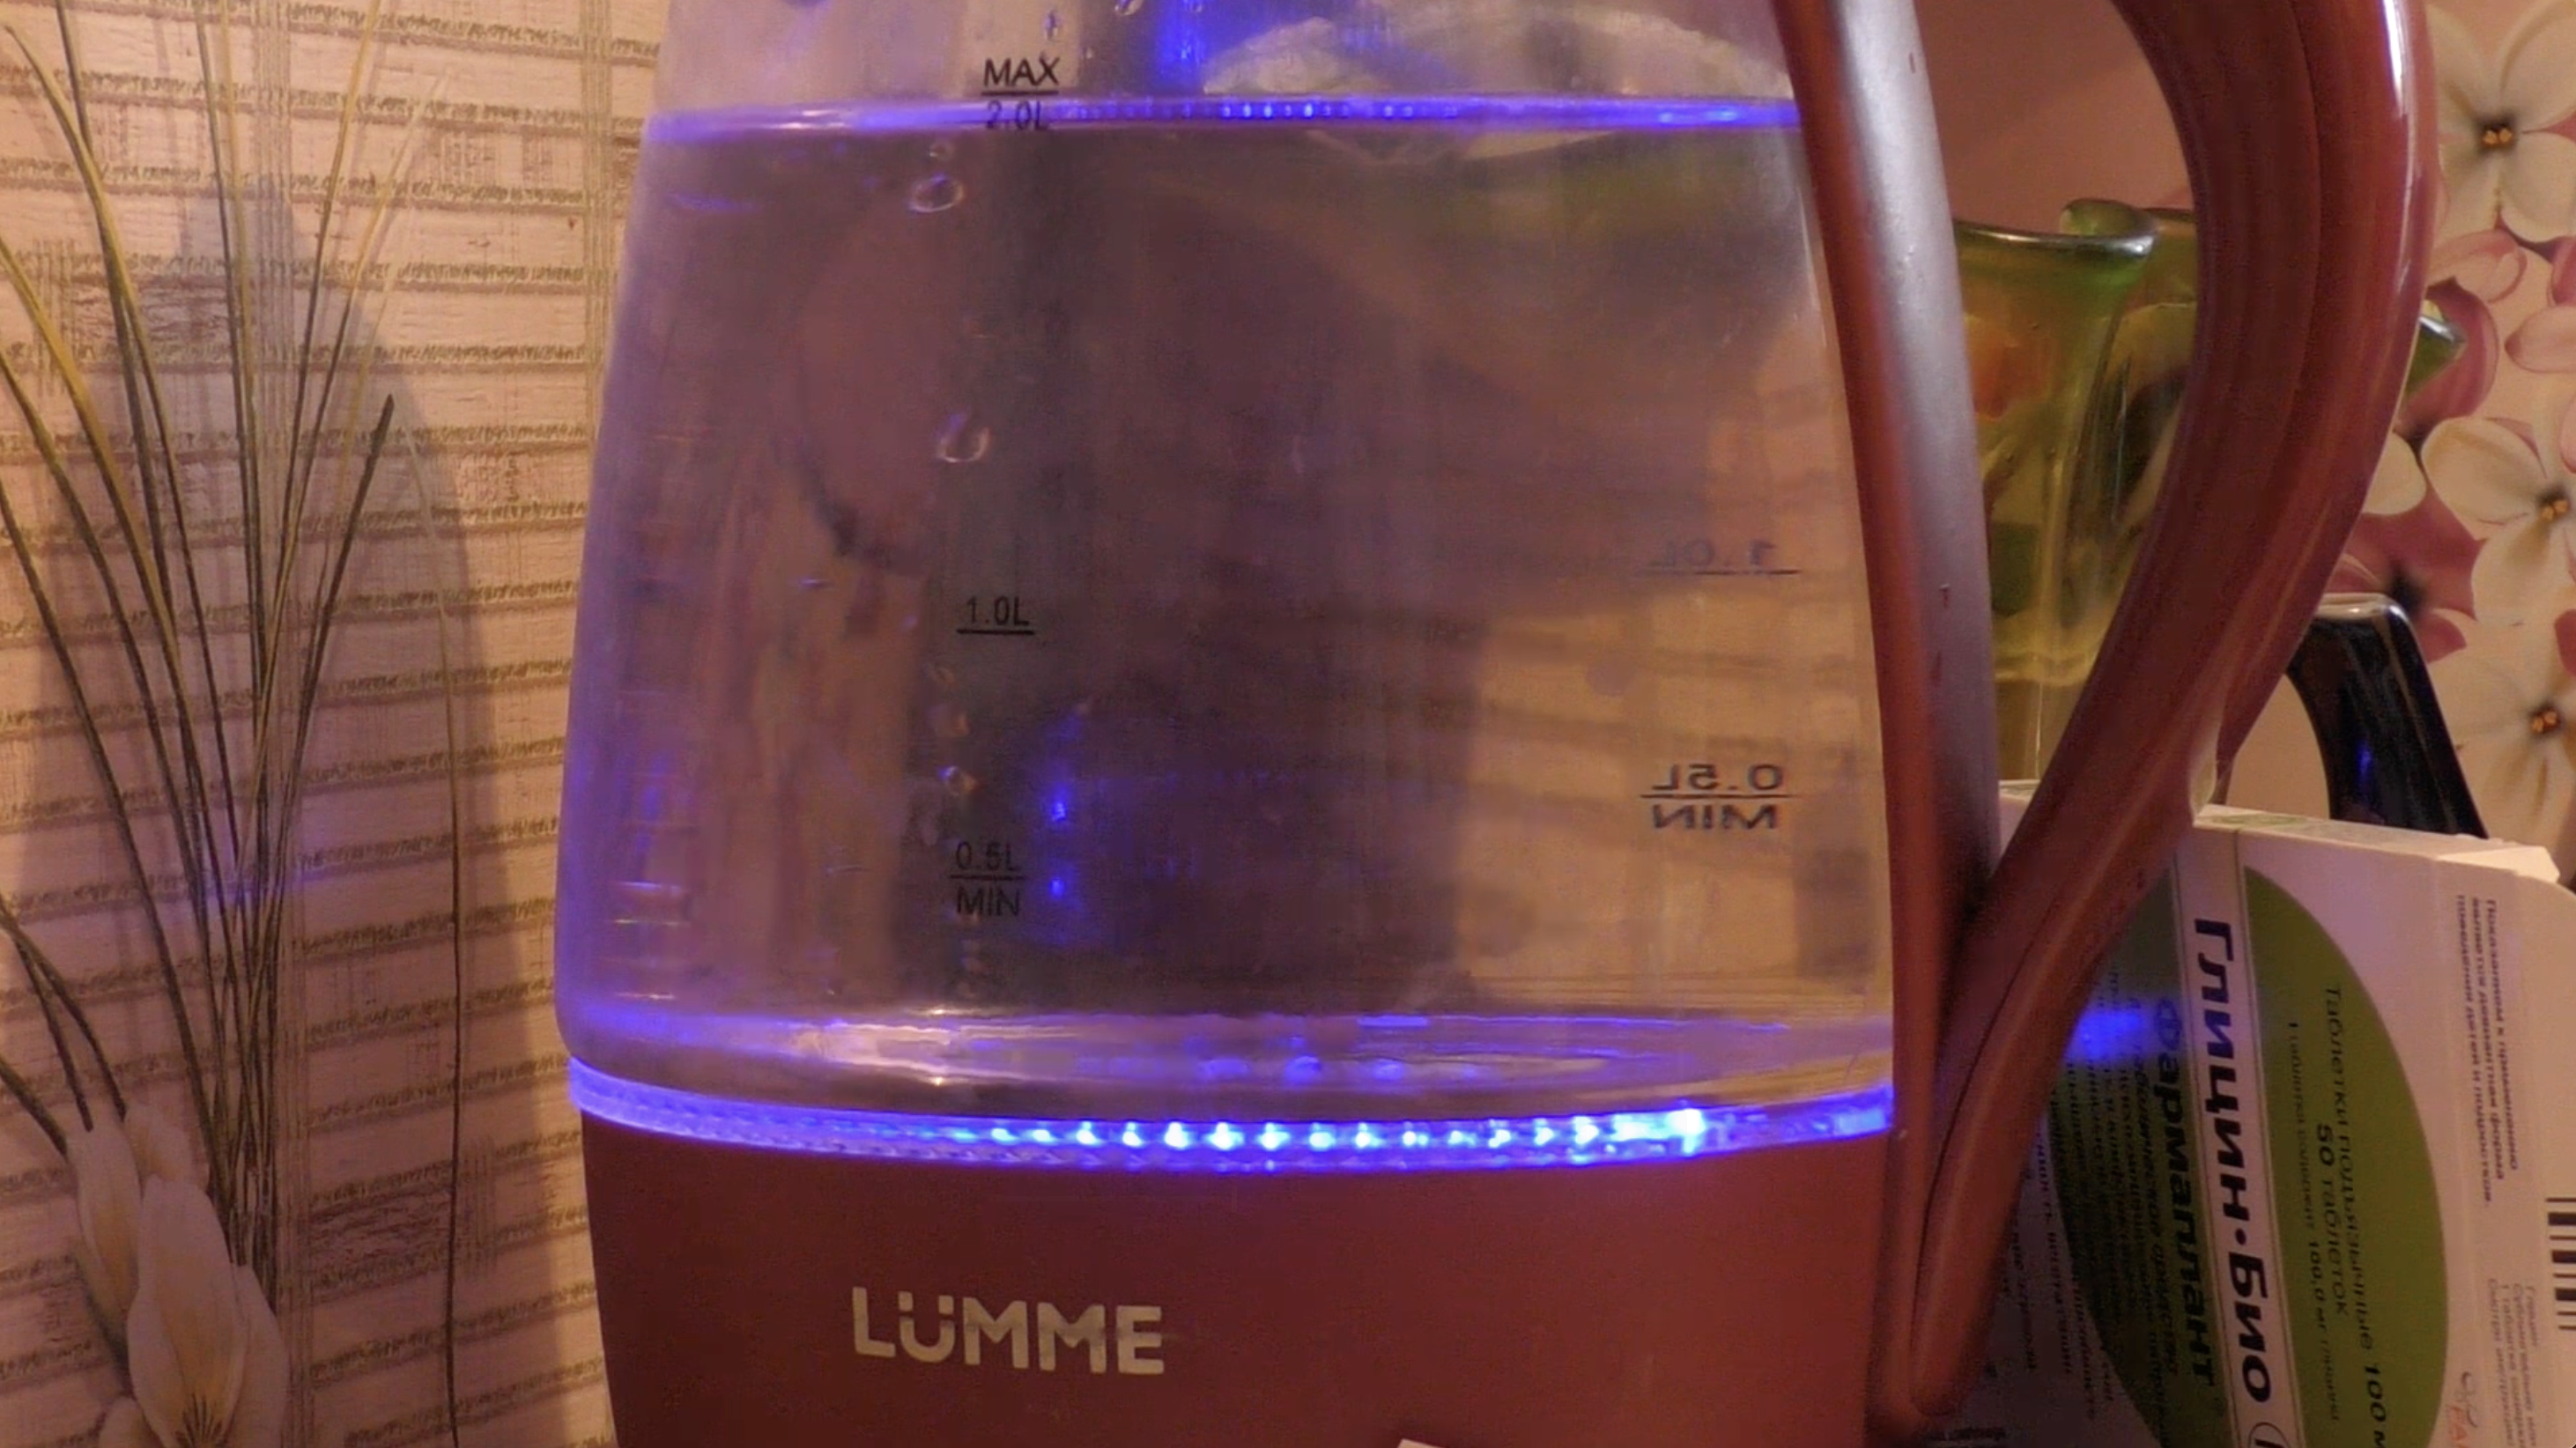
\includegraphics[width=0.70\linewidth]{img/image.png}
    \caption{Эталонный график функции }
\end{figure}

\newpage
\section{Ответ на контрольный вопрос}
\textbf{Вопрос: } Какие структуры используются для представления программ в ГП?
\textbf{Ответ: } 
\begin{itemize}
    \item \textbf{Древовидное представление:} Программа представляется в виде дерева, где листья (терминальные узлы) соответствуют переменным, константам или функциям без аргументов, а внутренние узлы — функциям (операторам).
    
    \item \textbf{Линейная структура:} Программа представляется в виде линейной последовательности операторов. Функциональное множество включает арифметические операции, условные операторы и вызовы функций, а терминальное — переменные и константы.
    
    \item \textbf{Графоподобная структура:} Программа представляется в виде графа. Это более общая структура, которая позволяет естественным образом моделировать операторы ветвления и циклы.
\end{itemize}

\newpage
\section*{Заключение}
\addcontentsline{toc}{section}{Заключение}
В результате выполнения лабораторной работы №4 были достигнуты следующие результаты:
\begin{itemize}
  \item освоен теоретический материал;
  \item создана программа на языке \texttt{Python} с использованием среды \texttt{Jupyter Notebook};
  \item реализован эволюционный алгоритм ГП для функции \(f_{1a}(\mathbf{x})=\sum_{i=1}^{n} i\,x_i^2\) и получены приближения на диапазоне \([-5.12,5.12]^9\);
  \item выполнена визуализация: срезы деревьев (10, 20, 50, 70, 100 поколения), финальное дерево, графики сходимости, среднего размера программ и распределения ошибок;
\end{itemize}

\newpage
\section*{Список литературы}
\addcontentsline{toc}{section}{Список литературы}
\begin{enumerate}
  \item Методические указания по выполнению лабораторных работ к курсу <<Генетические алгоритмы>>, стр.~119.
\end{enumerate}

\newpage
\addcontentsline{toc}{section}{Приложение А}
\twosideheading{Исходный код}{Приложение А}
\begin{lstlisting}
  import math
import random
import numpy as np
import matplotlib.pyplot as plt
from dataclasses import dataclass, field
from typing import Callable, List, Tuple, Union, Optional, Dict

try:
    import graphviz
    GRAPHVIZ_AVAILABLE = True
except Exception:
    GRAPHVIZ_AVAILABLE = False

SEED = 42
N_VARS = 9
DOMAIN = (-5.12, 5.12)
N_SAMPLES = 2000           
POP_SIZE = 300
GENERATIONS = 120
TOURNAMENT_K = 5
ELITE = 2
P_CROSS = 0.9
P_MUT_NODE = 0.2           
P_MUT_SHRINK = 0.1         
P_MUT_GROW = 0.2           
MAX_INIT_DEPTH = 6
MAX_TREE_DEPTH = 16
ERC_RANGE = (-5.0, 5.0)    
PLOT_EVERY = 10
LAMBDA_COMPLEXITY = 1e-4   
random.seed(SEED)
np.random.seed(SEED)

def p_div(x, y):
    denom = np.where(np.abs(y) < 1e-12, 1e-12, y)
    return x / denom

def p_pow(x, y):
    y_clip = np.clip(y, -4.0, 4.0)
    y_round = np.round(y_clip)
    is_int = np.isclose(y_clip, y_round)
    base = np.where(is_int, x, np.abs(x))
    try:
        out = np.power(base, np.where(is_int, y_round, y_clip))
    except FloatingPointError:
        out = np.power(np.clip(base, -1e6, 1e6), np.where(is_int, y_round, y_clip))
    return np.clip(out, -1e6, 1e6)

def p_exp(x):
    return np.exp(np.clip(x, -50, 50))

def p_sin(x):
    return np.sin(x)

def p_cos(x):
    return np.cos(x)

@dataclass(frozen=True)
class Primitive:
    name: str
    arity: int
    func: Callable

FUNCTIONS: List[Primitive] = [
    Primitive('+', 2, lambda a, b: a + b),
    Primitive('-', 2, lambda a, b: a - b),
    Primitive('*', 2, lambda a, b: a * b),
    Primitive('/', 2, p_div),
    Primitive('sin', 1, p_sin),
    Primitive('cos', 1, p_cos),
    Primitive('exp', 1, p_exp),
    Primitive('^', 2, p_pow),
]

@dataclass
class Terminal:
    kind: str
    index: Optional[int] = None
    value: Optional[float] = None

    def eval(self, X: np.ndarray) -> np.ndarray:
        if self.kind == 'var':
            return X[:, self.index]
        else:
            return np.full(X.shape[0], self.value, dtype=float)

    def __str__(self):
        if self.kind == 'var':
            return f"x{self.index+1}"
        else:
            return f"{self.value:.4g}"

@dataclass
class Node:
    prim: Union[Primitive, Terminal]
    children: List['Node'] = field(default_factory=list)

    def is_function(self) -> bool:
        return isinstance(self.prim, Primitive)

    def is_terminal(self) -> bool:
        return isinstance(self.prim, Terminal)

    def copy(self) -> 'Node':
        return Node(self.prim, [c.copy() for c in self.children])

    def depth(self) -> int:
        if self.is_terminal():
            return 1
        return 1 + max((ch.depth() for ch in self.children), default=0)

    def size(self) -> int:
        return 1 + sum(ch.size() for ch in self.children)

    def eval(self, X: np.ndarray) -> np.ndarray:
        if self.is_terminal():
            return self.prim.eval(X)
        args = [c.eval(X) for c in self.children]
        try:
            if self.prim.arity == 1:
                return self.prim.func(args[0])
            elif self.prim.arity == 2:
                return self.prim.func(args[0], args[1])
        except FloatingPointError:
            pass
        return np.full(X.shape[0], np.nan)

    def to_string(self) -> str:
        if self.is_terminal():
            return str(self.prim)
        name = self.prim.name
        if self.prim.arity == 1:
            return f"{name}({self.children[0].to_string()})"
        left = self.children[0].to_string()
        right = self.children[1].to_string()
        if name in ['+', '-', '*', '/', '^']:
            return f"({left} {name} {right})"
        return f"{name}({left}, {right})"

def random_terminal() -> Node:
    if random.random() < 0.5:
        idx = random.randrange(N_VARS)
        return Node(Terminal('var', index=idx))
    else:
        val = random.uniform(*ERC_RANGE)
        return Node(Terminal('erc', value=val))

def random_function(arity: Optional[int] = None) -> Primitive:
    if arity is None:
        return random.choice(FUNCTIONS)
    cands = [f for f in FUNCTIONS if f.arity == arity]
    return random.choice(cands)

def generate_full(depth: int) -> Node:
    if depth <= 1:
        return random_terminal()
    prim = random_function(arity=random.choice([1, 2]))
    return Node(prim, [generate_full(depth - 1) for _ in range(prim.arity)])

def generate_grow(depth: int) -> Node:
    if depth <= 1 or (depth > 1 and random.random() < 0.3):
        return random_terminal()
    prim = random_function(arity=random.choice([1, 2]))
    return Node(prim, [generate_grow(depth - 1) for _ in range(prim.arity)])

def generate_ramped(max_depth: int) -> Node:
    d = random.randint(2, max_depth)
    return generate_full(d) if random.random() < 0.5 else generate_grow(d)

def tournament(pop: List[Node], fitness: List[float], k: int) -> Node:
    idxs = random.sample(range(len(pop)), k)
    best = min(idxs, key=lambda i: fitness[i])  
    return pop[best].copy()

def all_nodes_with_parents(root: Node) -> List[Tuple[Optional[Node], int, Node]]:
    out = []
    def dfs(parent, idx, node):
        out.append((parent, idx, node))
        for i, ch in enumerate(node.children):
            dfs(node, i, ch)
    dfs(None, -1, root)
    return out

def replace_child(parent: Optional[Node], child_index: int, new_child: Node, root: Node) -> Node:
    if parent is None:
        return new_child
    parent.children[child_index] = new_child
    return root

def subtree_crossover(a: Node, b: Node, max_depth: int) -> Tuple[Node, Node]:
    a = a.copy()
    b = b.copy()
    a_nodes = all_nodes_with_parents(a)
    b_nodes = all_nodes_with_parents(b)
    _, _, a_sub = random.choice(a_nodes)
    _, _, b_sub = random.choice(b_nodes)

    a2 = a.copy()
    b2 = b.copy()
    astr = a_sub.to_string()
    bstr = b_sub.to_string()
    a2_nodes = all_nodes_with_parents(a2)
    b2_nodes = all_nodes_with_parents(b2)
    cand_a = [(p, i, n) for (p, i, n) in a2_nodes if n.to_string() == astr]
    cand_b = [(p, i, n) for (p, i, n) in b2_nodes if n.to_string() == bstr]
    if not cand_a or not cand_b:
        return a, b
    pa2, ia2, a_sub2 = random.choice(cand_a)
    pb2, ib2, b_sub2 = random.choice(cand_b)

    new_a = replace_child(pa2, ia2, b_sub2.copy(), a2)
    new_b = replace_child(pb2, ib2, a_sub2.copy(), b2)
    if new_a.depth() > max_depth or new_b.depth() > max_depth:
        return a, b
    return new_a, new_b

def mutate_node_replace(tree: Node) -> Node:
    t = tree.copy()
    parent, idx, node = random.choice(all_nodes_with_parents(t))
    if node.is_function():
        ar = node.prim.arity
        node.prim = random_function(arity=ar)
    else:
        node.prim = Terminal('var', index=random.randrange(N_VARS)) if random.random() < 0.5 \
                    else Terminal('erc', value=random.uniform(*ERC_RANGE))
    return t

def mutate_shrink(tree: Node) -> Node:
    t = tree.copy()
    funcs = [triple for triple in all_nodes_with_parents(t) if triple[2].is_function()]
    if not funcs:
        return t
    parent, idx, node = random.choice(funcs)
    return replace_child(parent, idx, random_terminal(), t)

def random_subtree(max_depth: int) -> Node:
    return generate_ramped(max_depth)

def mutate_grow(tree: Node, max_depth: int) -> Node:
    t = tree.copy()
    parent, idx, node = random.choice(all_nodes_with_parents(t))
    new_st = random_subtree(max_depth=min(5, max_depth))
    candidate = replace_child(parent, idx, new_st, t)
    if candidate.depth() > max_depth:
        return t
    return candidate

def target_function(X: np.ndarray) -> np.ndarray:
    idxs = np.arange(1, N_VARS + 1, dtype=float)
    return (X**2 @ idxs)

def make_dataset(n_samples: int, low: float, high: float) -> Tuple[np.ndarray, np.ndarray]:
    X = np.random.uniform(low, high, size=(n_samples, N_VARS))
    y = target_function(X)
    return X, y

def fitness_sse(ind: Node, X: np.ndarray, y: np.ndarray) -> float:
    pred = ind.eval(X)
    if np.any(np.isnan(pred)) or np.any(np.isinf(pred)):
        return 1e50
    err = y - pred
    sse = float(np.sum(err * err))
    if LAMBDA_COMPLEXITY > 0:
        sse += LAMBDA_COMPLEXITY * (ind.size() ** 2)
    return sse

def plot_tree_graphviz(root: Node, filename: str, title: Optional[str] = None):
    if not GRAPHVIZ_AVAILABLE:
        return
    dot = graphviz.Digraph(comment=title or 'tree', format='png')
    def add(node: Node) -> str:
        node_id = str(id(node))
        if node.is_terminal():
            label = str(node.prim)
            shape = 'box'
            fill = 'honeydew'
        else:
            label = node.prim.name
            shape = 'ellipse'
            fill = 'lightsteelblue'
        dot.node(node_id, label, shape=shape, style='filled', fillcolor=fill)
        for ch in node.children:
            ch_id = add(ch)
            dot.edge(node_id, ch_id)
        return node_id
    add(root)
    out = dot.render(filename, view=False)
    print(f"[Graphviz] {out}")

def evolve():
    X, y = make_dataset(N_SAMPLES, *DOMAIN)
    X_val, y_val = make_dataset(1000, *DOMAIN)
    pop = [generate_ramped(MAX_INIT_DEPTH) for _ in range(POP_SIZE)]
    fitness = [fitness_sse(ind, X, y) for ind in pop]
    sizes = [ind.size() for ind in pop]

    best_idx = int(np.argmin(fitness))
    best = pop[best_idx].copy()
    best_fit = fitness[best_idx]

    best_hist = [best_fit]                
    avg_size_hist = [float(np.mean(sizes))] 

    print(f"Init best SSE: {best_fit:.6g} | depth={best.depth()} | size={best.size()}")
    print("Best expr:", best.to_string())

    for gen in range(1, GENERATIONS + 1):
        new_pop: List[Node] = []

        elite_idx = np.argsort(fitness)[:ELITE]
        for ei in elite_idx:
            new_pop.append(pop[ei].copy())

        while len(new_pop) < POP_SIZE:
            if random.random() < P_CROSS and len(new_pop) + 1 < POP_SIZE:
                p1 = tournament(pop, fitness, TOURNAMENT_K)
                p2 = tournament(pop, fitness, TOURNAMENT_K)
                c1, c2 = subtree_crossover(p1, p2, MAX_TREE_DEPTH)
                new_pop.extend([c1, c2])
            else:
                p = tournament(pop, fitness, TOURNAMENT_K)
                c = p
                if random.random() < P_MUT_NODE:
                    c = mutate_node_replace(c)
                if random.random() < P_MUT_SHRINK:
                    c = mutate_shrink(c)
                if random.random() < P_MUT_GROW:
                    c = mutate_grow(c, MAX_TREE_DEPTH)
                new_pop.append(c)

        pop = new_pop[:POP_SIZE]
        fitness = [fitness_sse(ind, X, y) for ind in pop]
        sizes = [ind.size() for ind in pop]

        gen_best_idx = int(np.argmin(fitness))
        gen_best = pop[gen_best_idx]
        gen_best_fit = fitness[gen_best_idx]
        if gen_best_fit < best_fit:
            best_fit = gen_best_fit
            best = gen_best.copy()

        best_hist.append(best_fit)
        avg_size_hist.append(float(np.mean(sizes)))

        if gen % 1 == 0:
            print(f"Gen {gen:4d} | best SSE={best_fit:.6g} | depth={best.depth():2d} | size={best.size():4d} | avg_size={avg_size_hist[-1]:.1f}")
        if gen % PLOT_EVERY == 0:
            title = f"Gen {gen} | SSE(val)={fitness_sse(best, X_val, y_val):.4g}"
            plot_tree_graphviz(best, filename=f"tree_gen_{gen}", title=title)

    final_sse_train = fitness_sse(best, X, y)
    final_sse_val = fitness_sse(best, X_val, y_val)

    plot_tree_graphviz(best, filename='tree_final', title=f"FINAL | SSE(val)={final_sse_val:.4g}")

    plt.figure(figsize=(7,4.5))
    plt.plot(best_hist, linewidth=2)
    plt.grid(True, alpha=0.3)
    plt.tight_layout()
    plt.show()

    plt.figure(figsize=(7,4.5))
    plt.plot(avg_size_hist, linewidth=2)
    plt.xlabel("Evo")
    plt.ylabel("Mean")
    plt.title("Tree cap")
    plt.grid(True, alpha=0.3)
    plt.tight_layout()
    plt.show()

    yhat_val = best.eval(X_val)
    residuals = y_val - yhat_val
    plt.figure(figsize=(7,4.5))
    plt.hist(residuals, bins=50, alpha=0.8)
    plt.xlabel("Err")
    plt.ylabel("Val")
    plt.title("Valid")
    plt.grid(True, alpha=0.3)
    plt.tight_layout()
    plt.show()

if __name__ == "__main__":
    evolve()
\end{lstlisting}
\end{document}